\input ../talk-header.tex
\title
{Machine Learning}
\subtitle{Features and Modeling}

\begin{document}

\maketitle

\begin{frame}
  \vspace{4mm}
  
  \cimgh{titanic-titles.png}
  \vspace{-3mm}
  \prevwork{Kaggle}
\end{frame}

\begin{frame}
  \cimg{reading-time-1.png}
  \prevwork{Jellybooks}
\end{frame}

\begin{frame}
  \cimg{reading-time-2.png}
  \prevwork{Jellybooks}
\end{frame}

\begin{frame}
  \frametitle{pandas}
  \only<1>{\lstinputlisting{pandas_1.py}}
  \only<2>{\purple{\texttt{Dataframe} has many constructors.  For example,}
    \lstinputlisting{pandas_2.py}
  }
  \only<3>{\purple{Viewing data}
    \lstinputlisting{pandas_3.py}
  }
  \only<4>{\purple{Basic data exploration}
    \lstinputlisting{pandas_4.py}
  }
  \only<5>{\purple{Select a column (series)}
    \lstinputlisting{pandas_5.py}
  }
  \only<6>{\purple{Select a range}
    \lstinputlisting{pandas_6.py}
  }
  \only<7>{\purple{Boolean selection criteria}
    \lstinputlisting{pandas_7.py}
  }
  \only<8>{\purple{Recommended}
    
    \vspace{5mm}
    \url{http://www.gregreda.com/2013/10/26/intro-to-pandas-data-structures/}
  }
\end{frame}

\begin{frame}
  \frametitle{Plotting}
  \only<1>{\purple{Draw a line}
    \lstinputlisting{pyplot_1.py}
    \vspace{-19mm}
    \flushright{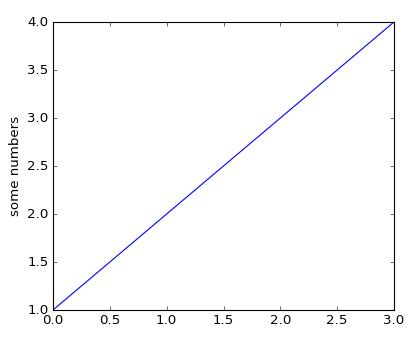
\includegraphics[width=.5\textwidth]{pyplot_1.png}}
  }
  \only<2>{\purple{Draw a line}
    \lstinputlisting{pyplot_2.py}
    \vspace{-19mm}
    \flushright{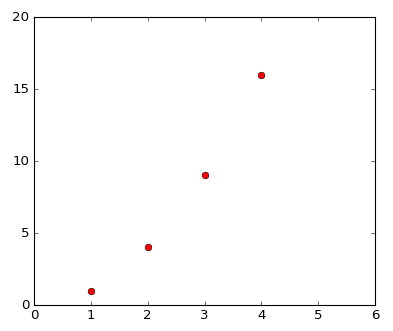
\includegraphics[width=.5\textwidth]{pyplot_2.png}}
  }
  \only<3>{\purple{Draw a line}
    \lstinputlisting{pyplot_3.py}
    \vspace{-55mm}
    \flushright{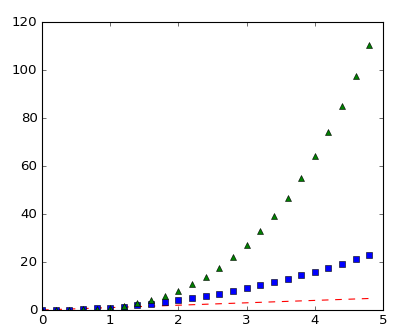
\includegraphics[width=.5\textwidth]{pyplot_3.png}}
  }
  \only<4>{\purple{Draw two curves}
    \lstinputlisting{pyplot_4.py}
  }
  \only<5>{
    \flushright{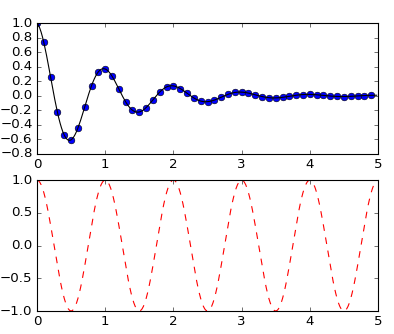
\includegraphics[width=.5\textwidth]{pyplot_4.png}}
  }    
  \only<6>{\purple{Draw two curves}
    \lstinputlisting{pyplot_5.py}
  }
  \only<7>{
    \flushright{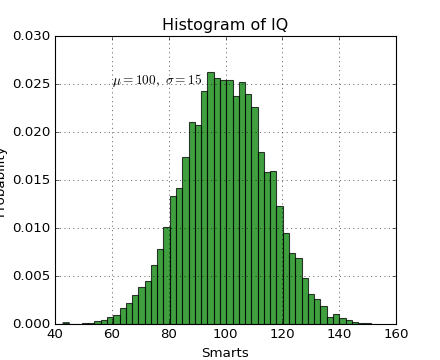
\includegraphics[width=.5\textwidth]{pyplot_5.png}}
  }
  \only<8>{\purple{Scatter plot}
    \prevwork{\url{http://matplotlib.org/mpl_examples/pylab_examples/scatter_demo2.py}}
    \lstinputlisting{pyplot_6.py}
    \vspace{-60mm}
    \flushright{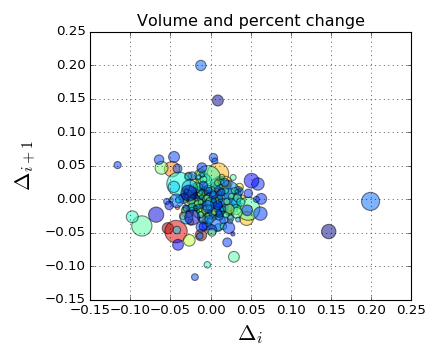
\includegraphics[width=.5\textwidth]{pyplot_6.png}}
    
  }
  \only<9>{
    \prevwork{\url{http://matplotlib.org/users/pyplot_tutorial.html}}
      
    \prevwork{\url{http://matplotlib.org/users/beginner.html}}
  }
\end{frame}

\end{document}
